\begin{figure}
	\centering
	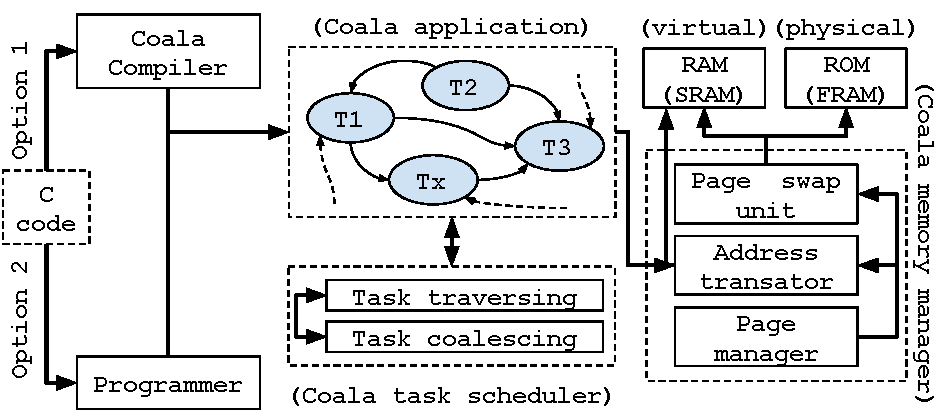
\includegraphics[width=\columnwidth]{figures/viper_block_diagram}
	\caption{\sys top-level view.}
	\label{fig:system_overview}
\end{figure}

\sys as a whole is characterized by the following features:

\begin{itemize}
	\item \textbf{Task coalescing}: details will be provided in Section~\ref{sec:task_coalescing}
	\item \textbf{Memory virtualization}: details will be provided in Section~\ref{sec:memory_virtulaization}
	\item \textbf{Compiler support}: details will be provided in Section~\ref{sec:compiler}
\end{itemize}

A complete logical structure of \sys is given in Figure~\ref{fig:system_overview}. Before describing each feature of \sys in detail we need to introduce a programming and semantics/execution model.

\begin{figure}
	\centering
	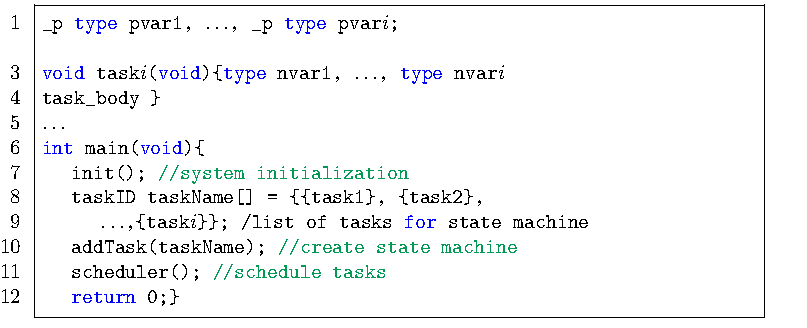
\includegraphics[width=\columnwidth]{figures/taskification_example}
	\caption{\sys API.}
	\label{fig:system_overview}
\end{figure}


\subsection{Programming Model}
\label{sec:overview_programming_model}



\subsection{Semantics and Execution Model}
\label{sec:overview_semantics}

